\chapter{Projekt}
Rozdział ten zawiera szkice rozwiązań dla wymagań z~poprzednich rozdziałów.

\section{Podział na warstwy}
Zdecydowałem się podzielić wykres na pięć warstw. Odrysowywanie wykresu będzie się składało z~odrysowania zawartości każdej z~warstw, począwsze od tła, a~na pierwszym planie skończywszy.
Układ warstw został przedstawiony na rysunku~\ref{rys:warstwy}.

\begin{figure}[H]
\centering
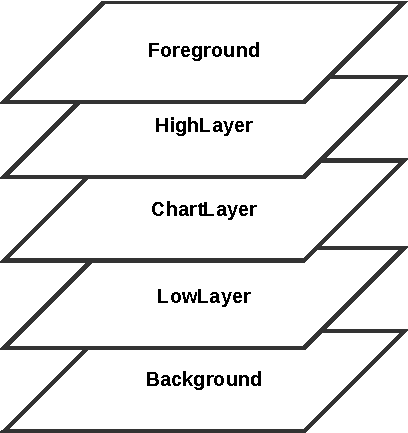
\includegraphics{img/warstwy.pdf}
\caption{Warstwy wykresu}\label{rys:warstwy}
\end{figure}

Warstwy tła oraz pierwszego planu służą jedynie odrysowywaniu wzorów przekazanych za pomocą pędzla. Pozostałe warstwy są bardziej złożone i~zawierają liczne elementy.

Warstwy niska i~wysoka są odrysowywane zgodnie z~algorytmem malarza. Służą dodawaniu przez programistów własnych elementów do wykresów istniejących klas.

Warstwa wykresu służy odrysowaniu głównej zawartości wykresu. Tym etapem steruje strategia danego wykresu. W~ogólnym przypadku programiści nie powinni dodawać własnych elementów do tej warstwy.

%\subsection{Metoda szablonowa}
Metoda odpowiedzialna za odrysowywanie wykresu powinna być \textit{Metodą Szablonową}~\cite{Patterns}, czyli niewirtualną, publiczną metodą klasy bazowej, wywołującą kolejne metody odpowiedzialne za odrysowanie pojedynczych warstw. Metody te powinny z~kolei być wirtualne i~chronione.
Metody odpowiedzialne za tło i~pierwszy plan powinny udostępniać domyślną implementację, natomiast pozostałe powinny być czysto wirtualne.

\section{Lokalny układ współrzędnych}
Każdy z~wykresów będzie posiadać lokalny, kartezjański układ współrzędnych rzeczywistych. Ponadto granice wykresu będą wyznaczane przez specjalny prostokąt. Takie podejście umożliwi układanie elementów względem lokalnego, a~nie globalnego układu współrzędnych, oraz ustalanie, które z~elementów są widoczne i~należy je odrysować. Dodatkowo ułatwiona będzie realizacja takich wymagań jak: skalowanie wykresu czy interaktywność. 

\begin{figure}[H]
\centering
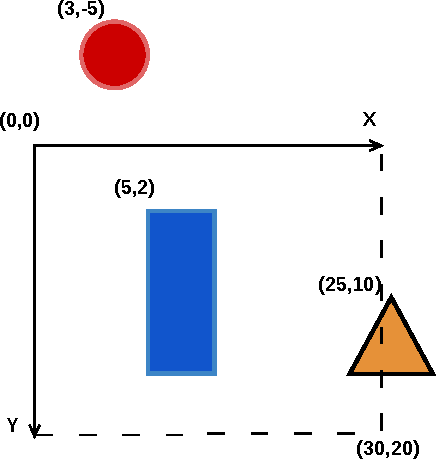
\includegraphics{img/uklad_wspolrzednych.pdf}
\caption{Lokalny układ współrzędnych}\label{rys:uklad:wspolrzednych}
\end{figure}

Na rysunku~\ref{rys:uklad:wspolrzednych} przedstawiono przykładowy układ współrzędnych wykresu o~wymiarach 30x20. W~tej sytuacji prostokąt zostanie wyświetlony w~całości, trójkąt tylko częściowo, a~koło wcale nie zostanie wyświetlone.

\section{Diagramy klas}

\subsection{Top level}
Ogólna koncepcja na strukturę wykresu została przedstawiona na diagramie~\ref{rys:klasy:top_level}.

Klasy pochodne od QocAbstractChart są miejscem łączącym wszystkie inne elementy. To na nich będą ustawiane parametry odnoszące się do całości wykresu, np. włączenie antyaliasingu.

QocSeries odpowiada za dane dostarczane do wykresu. Jest lekkim odpowiednikiem modelu z~architektury Model-Widok.

QocAbstractStrategy to klasa bazowa dla strategii -- layoutu, odpowiedzialnego za odpowiednie układanie elementów wykresu, głównie z~warstwy środkowej -- \textit{ChartLayer}, i~ich odrysowywanie. Jest to szczególnie przydatny komponent dla wykresów, które mogą być budowane na różne sposoby, np. wykres słupkowy.


\begin{figure}[H]
\centering
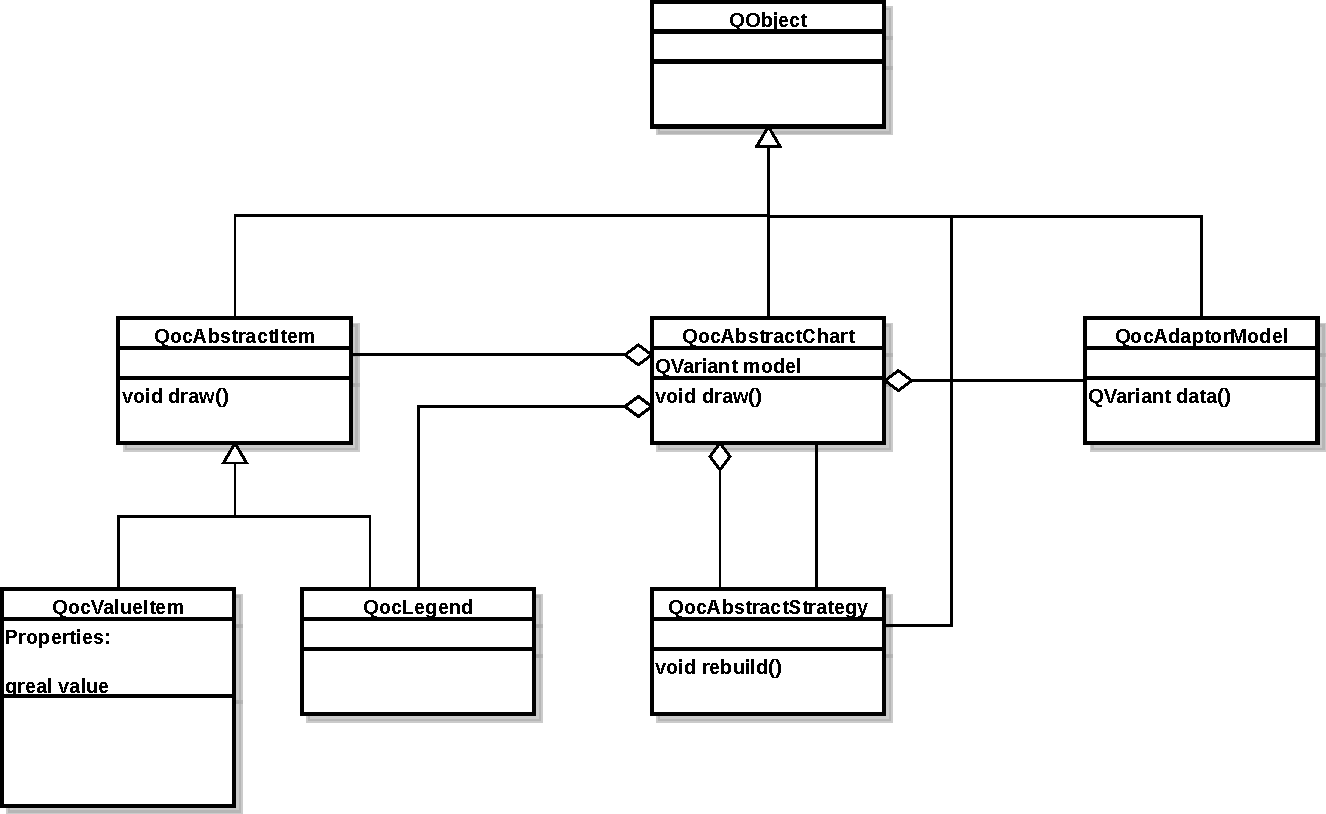
\includegraphics[scale=0.7]{img/klasy-top_level.pdf}
\caption{Diagram top level}\label{rys:klasy:top_level}
\end{figure}

\section{Źródła danych}

Jako że źródłem danych dla wykresu może być seria danych, zbiór serii albo model, postanowiłem wprowadzić pośrednią klasę, która będzie odpowiedzialna za unifikację komunikacji wykresu ze źródłem danych. Klasa ta będzie \textit{Adapterem obiektowym}~\cite{Patterns} -- będzie agregowała źródła danych dostarczane jako obiekty \textit{QVariant}. Hierarchię klas związanych z~adapterem przedstawiłem na diagramie~\ref{rys:adapter:model}

\begin{figure}[H]
\centering
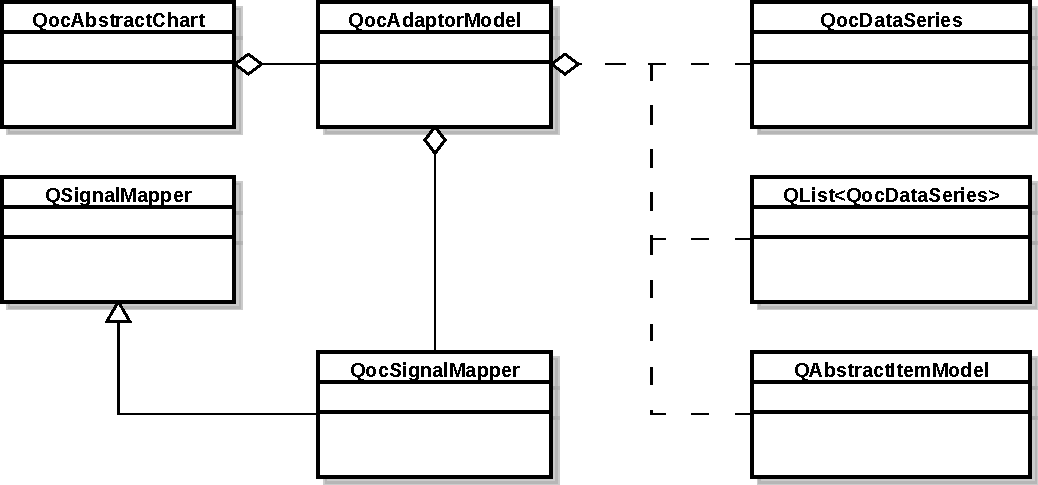
\includegraphics[scale=0.8]{img/adapter-model.pdf}
\caption{Adapter}\label{rys:adapter:model}
\end{figure}

Za pomocą adaptera stworzę pewną abstrakcję, dzięki której niezależnie od klasy źródła danych, wykres zawsze będzie go postrzegał jako zbiór serii. Większość metod adaptera, jako jeden z~argmuentów będzie przyjmować identyfikator serii, dzięki czemu będzie można wyspecyfikować  której serii dotyczy dana operacja. 

Komunikacja w~drugą stronę zostanie rozwiązana za pomocą zbioru sygnałów, które również będą niosły informację o~id serii. W~przypadku zbioru serii, wystarczy uzupełnić ich sygnały o~id serii oraz przepropagować na zewnątrz adaptera. Chcę to osiągnąć za pomocą obiektu klasy pochodnej od \textit{QSignalMapper}~\footnote{QSignalMapper \url{http://qt-project.org/doc/qt-5.0/qtcore/qsignalmapper.html}}. W~przypadku klas modeli, również będę musiał wykonać podobne mapowanie, podczas którego trzeba będzie sięgnąć do modelu po id serii. Przykładowy protokół komunikacji wykresu z~adapterem przedstawiłem na rysunku~\ref{rys:wykres:model}.

\begin{figure}[H]
\centering
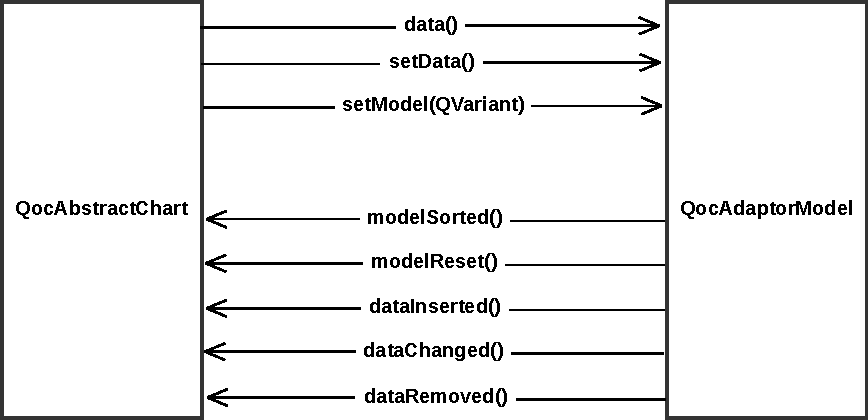
\includegraphics[scale=0.8]{img/wykres-model.pdf}
\caption{Komunikacja Wykres -- Adapter}\label{rys:wykres:model}
\end{figure}

\subsection{Role}
Wzorując się na systemie Model-Widok, zdecydowałem się wprowadzić do mojej biblioteki byt o~nazwie: Rola. Rola to wartość enumeryczna, która służy wskazania przez widok, jakich danych oczekuje od modelu. Widok chcąc uzyskać dane z~modelu musi mu przekazać indeks i~właśnie rolę.

Dzięki rolom uzyskam sytuację, w~której wykres chcąc pobrać dane z~modelu, przekaże do adaptera rolę. Adapter zajmie się przetłumaczeniem roli. W~zależności od kontekstu, może to być numer kolumny albo właściwość obiektu.

\begin{lstlisting}
enum Role{
	SeriesIndexRole,
	XRole,
	YRole,
	TitleRole,
	ColorRole,
	CustomRole
}
\end{lstlisting}

\subsection{QAbstractItemModel}
Pracując na seriach danych, które są mojego autorstwa, mogę założyć, że dla elementu o~danym indeksie i~roli wartość jest, np. tytułem zapisanym w~łańcuchu znaków. Takiego komfortu jednak nie będzie przy współpracy z~dowolnym innym modelem. Nie mogę wymagać od użytkownika, aby interesujące mnie dane trzymał w~kolumnach o~ustalonych przeze mnie indeksach. Rozwiązaniem tej sytuacji mogłoby być stworzenie specjalnego proxy modelu~\footnote{Proxy modele \url{http://qt-project.org/doc/qt-5.0/qtcore/qabstractproxymodel.html}}, jednak preferuję inny sposób.

Moje rozwiązanie polega na mapowaniu ról, które są zrozumiałe dla wykresów, na numery kolumn modeli do tych wykresów podłączanych. Z~perspektywy programisty mapowanie powinno się ograniczać jedynie do wywołania poniższej metody dla wszystkich wymagających tego ról:

\begin{lstlisting}
QocAbstractChart::setRoleMapping(Qoc::Role role, int customValue);
\end{lstlisting}

Metoda ta przyjmuje jako pierwszy z~argumentów rolę, a~jako drugi numer kolumny, pod którą kryją się odpowiednie dane w~modelu. Metoda ta będzie pomocna również przy współpracy z~modelami QML.


\subsection{QML}
ListModel i XmlListModel to pochodne QAbstractItemModel, które należy potraktować osobno. Wprowadzają one bardziej obiektowe podejście, dzięki czemu ich zawartość jest łatwo dostępna z~QML.

Dane z~tych modeli są dostępne również poprzez system właściwości. Aby dostać się do wartości właściwości wystarczy jedynie znać jej nazwę. Dzięki temu, wymuszając na użytkownikach określone nazwy właściwości, jestem w~stanie pobierać dane z~ich modeli. W~skrajnym przypadku, gdy programista korzystający z~mojej biblioteki nie będzie mógł dostarczyć danych w~oczekiwanym przeze mnie formacie, udostępniam mu przeładowaną metodę z~poprzedniego podpunktu:

\begin{lstlisting}
QocAbstractChart::setRoleMapping(Qoc::Role role, const QString &name);
\end{lstlisting}

W~tym przypadku jako drugi argument przyjmuję nową nazwę danej właściwości. Po wywołaniu metody, nowa nazwa właściwości będzie wykorzystywana do komunikacji z~modelem.


\section{Qt Quick}

\subsection{Eksport klas C++ do QML}
Klasy wszystkich wysokopoziomowych elementów powinny być pochodnymi klasy QObject. Wszelkie ich parametry, które powinny być konfigurowane przez programistów należy włączyć do zbioru właściwości tej klasy. W~szczególności należy zadbać o~to, aby przy zmianie wartości danej właściwości, i~tylko wtedy, emitować sygnał informujący o~tym zdarzeniu. Jest to niezbędne do poprawnego działania mechanizmu wiązania w~QML. Ponadto, wszystkie metody, które powinny być dostępne z~QML, a~nie są slotami, powinny zostać opatrzone makrem \textit{Q\_INVOKABLE}.

Większość klas powinna być gotowa do wyeksportowania ich do QML za pomocą standardowej procedury, np. poprzez wywołanie funkcji szablonowej
\begin{verbatim}
template<typename T>
int qmlRegisterType(const char *uri, int versionMajor, 
		    int versionMinor, const char *qmlName)
\end{verbatim}
Parametrem szablonu jest eksportowany typ, a~parametry funkcji to nazwa modułu, dwie liczby odpowiadające za wersję modułu oraz nazwa pod jaką będzie dostępna eksportowana klasa z~poziomu QML. Qt udostępnia jeszcze kilka innych, specjalizowanych szablonów, np. dla singletonów.

Pozostałe klasy, do wykorzystania ich w~QML, będą wymagały specjalnych interfejsów. Dla klas związanych z~GUI, bazujących na QPainter będzie to QQuickPaintedItem, a~dla tych wykorzystujących SceneGraph -- QQuickItem.

\subsection{Uproszczony interfejs}
Zakładam, że w~niektórych przypadkach interfejsy dostępne z~poziomu QML mogą, a~nawet powinny być uboższe od swoich odpowiedników w~C++. Najlepszym przykładem będzie ramka wokół dowolnego elementu graficznego, będącego składową wykresu. Z~poziomu C++ powinna istnieć możliwość ustawienia pióra używanego do jej odrysowania. Klasa pióra, czyli \textit{QPen}, nie dziedziczy po \textit{QObject}, więc nie może być dostępna w~QML.

Jednym z~rozwiązań tego problemu jest stworzenie specjalnych adapterów dla wszystkich klas nie spokrewnionych z~\textit{QObject}, które wykorzystam w~swojej bibliotece. Wolę jednak przyjąć konwencję stosowaną w~Qt~Quick i~ograniczyć, uprościć interfejsy moich klas dla QML, tak aby możliwe było tam zmienianie tylko najważniejszych parametrów. W~przypadku ramki będą to grubość oraz kolor. Jednocześnie z~poziomu C++ cały czas będzie można zmienić wszystkie parametry pióra odrysowujacego daną ramkę.

\section{Interaktywność}
%Klasy wykresów muszą udostępniać metody mapujące globalne współrzędne na wartości lokalne i~odwrotnie. Ponadto każdy z~elementów wykresu musi posiadać metody:
%\begin{itemize}
%\item{boundingRect(), zwracająca najmniejszy prostokąt opisujący dany element.}
%\item{shape(), zwracająca kształt elementu zapisany jako \textit{QPainterPath}.}
%\end{itemize}

\subsection{Zmiana wartości w modelu}
Na rysunku~\ref{rys:seq:inter} przedstawiam diagram sekwencji dotyczący zmiany zawartości modelu poprzez modyfikację elementów widoku. Przerywane strzałki zawierające opis symbolizują wywołanie sygnału.

\begin{figure}[H]
\centering
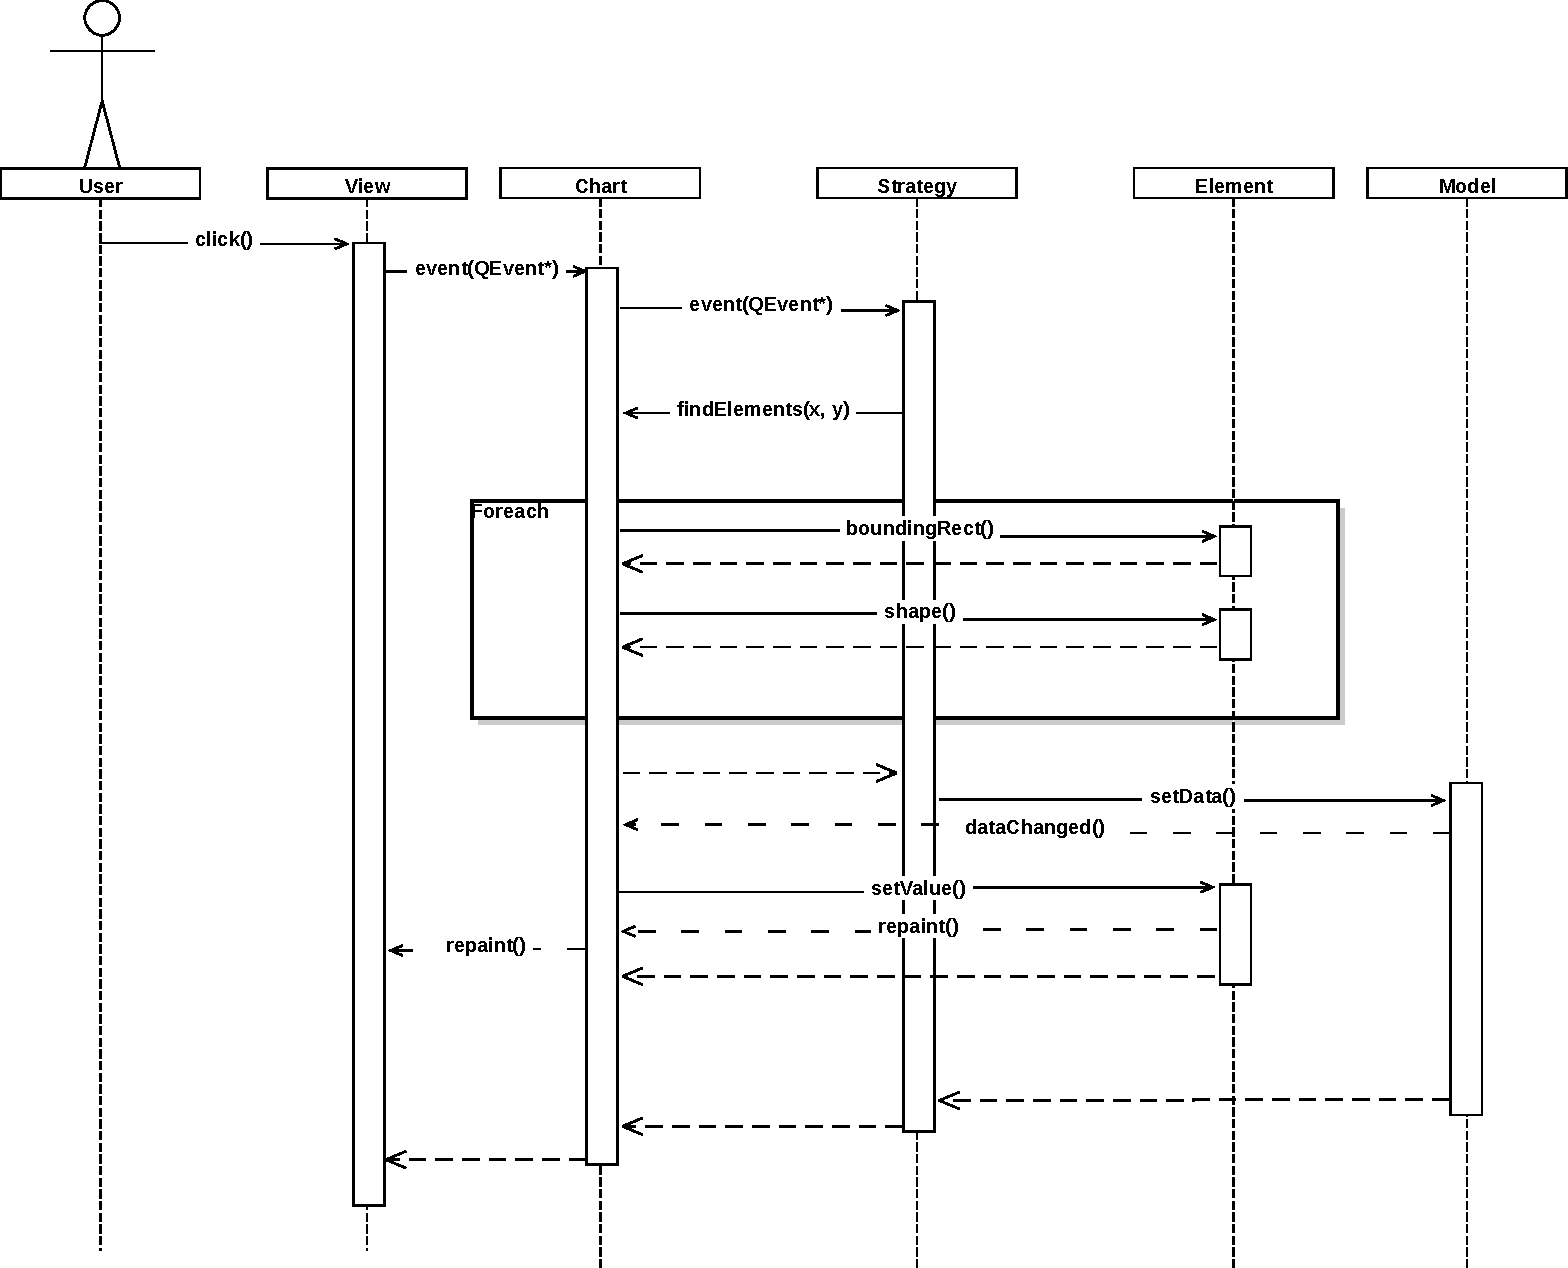
\includegraphics[scale=0.6]{img/seq_inter.pdf}
\caption{Interaktywna zmiana zawartości modelu}\label{rys:seq:inter}
\end{figure}

\section{Współpraca wykresów z widokami }
Jak już zostało ustalone, celem tworzonej biblioteki jest stworzenie uniwersalnego silnika, umożliwiającego tworzenie wykresów gotowych do podpięcia do jednego z~kilku widoków. Na rysunku~\ref{rys:widok:wykres} przedstawiłem składniki protokołu komunikacji między widokiem a dowolnym wykresem z~mojej biblioteki.

Widok ma obowiązek przesyłać do wykresu wszelkie zdarzenia, które są dla niego przeznaczone oraz informować wykres o~zmianach swojej geometrii. Ponadto przy odrysowywaniu widok musi wywoływać metodę \textit{draw()} wykresu.

Wykres nie powinien posiadać informacji z~widokiem jakiej klasy współpracuje. Można to osiągnać za pomocą mechanizmu sygnałów i~slotów, który pozwala na luźne wiązanie elementów. Odpowiednie sygnały  powinny być emitowane przez wykres zawsze wtedy, gdy wymaga on ponownego odrysowania.
Sygnał \textit{repaint()} powinien być emitowany w~sytuacji gdy ponowne odrysowanie musi nastąpić niemal natychmiast, natomiast sygnał \textit{update()} jest przeznaczony na sytuacje gdy zgłoszenia odrysowania mogą zostać skolejkowane, sklejone i~obsłużone jako jedno zgłoszenie w~najbliższej wolnej chwili.


\begin{figure}[H]
\centering
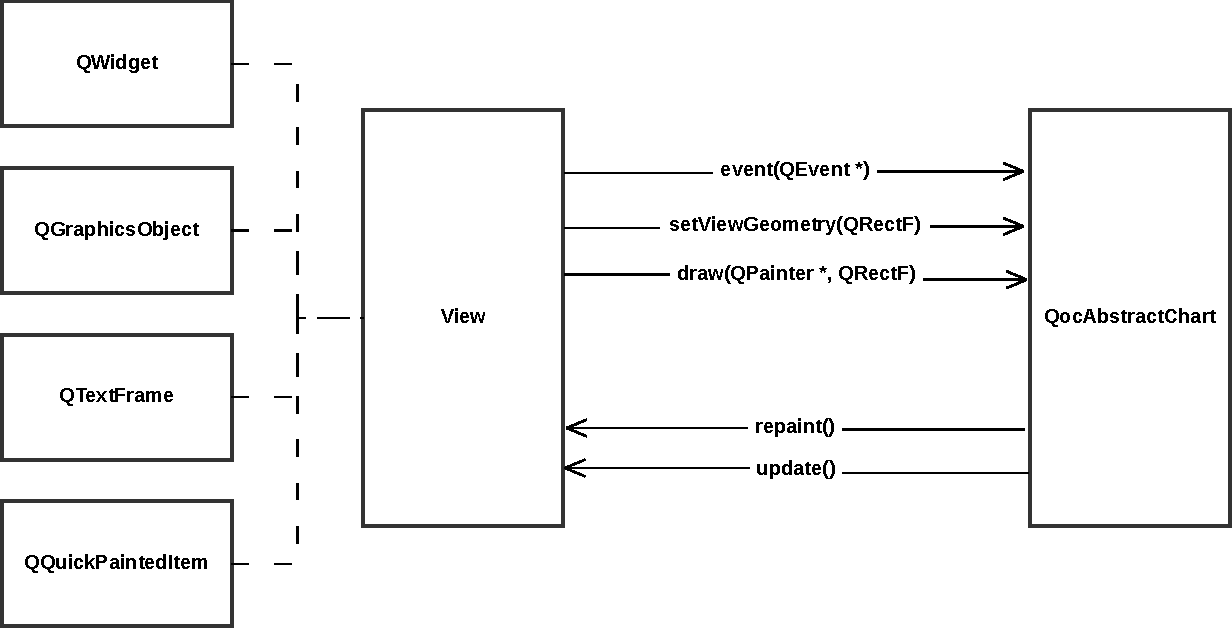
\includegraphics[scale=0.75]{img/widok-wykres.pdf}
\caption{Widok -- Wykres}\label{rys:widok:wykres}
\end{figure}

%\subsubsection{Wskazówki implementacyjne}
%Klasa bazowa wykresów powinna posiadać właściwość typu prostokąt, opisującą geometrię widoku podłączonego do danego wykresu. Zmiana tej właściwości powinna się odbywać poprzez odpowiedni slot, przyjmujący jako argument nowy prostokąt.

%W~zależności od klasy, z~której wywodzi się widok podłączony do wykresu, slot powiadamiający wykres o~zmianie geometrii widoku powinien być wywoływany następujących metodach widoku:
%\begin{itemize}
%\item{QWidget}
%	\begin{itemize}
%	\item{moveEvent()}
%	\item{resizeEvent()}
%	\end{itemize}
%\item{QGraphicsObject}
%	\begin{itemize}
%	\item{prepareGeometryChange()}
%	\end{itemize}
%\item{QTextFrame}

%\item{QQuickPaintedItem}
%	\begin{itemize}
%	\item{geometryChanged()}
%	\end{itemize}
%\end{itemize}

\section{Zależności między plikami}
Mogłoby się wydawać, że każde nowe wydanie Qt powinno wymagać ponownej kompilacji projektów zeń korzystających. Tak jednak nie jest. Twórcy Qt zadbali o~to, aby zawsze wtedy, kiedy to możliwe, zachowana była zgodność binarna. Oznacza to, że jeśli przy poprawkach do nowej wersji nie zostały zmienione nagłówki klas, a~jedynie ich implementacje, to przebudowanie całej aplikacji nie jest konieczne. Teoretycznie przejście z~Qt~w~wersji 4.8.3 na wersję 4.8.4 może odbyć się jedynie poprzez podmianę plików .dll. Temat zgodności binarnej oraz zależności czasu kompilacji między plikami został poruszony przez Scotta Meyersa~\cite{50Ways}.

\subsection{QObject}
Klasa QObject została zaprojektowana jako \textit{Most}~\cite{Patterns}.
%, zmodyfikowany o~posiadany przez ciało wskaźnik do uchwytu. 
Podział na uchwyt i~ciało zmniejsza zależności pomiędzy plikami bibliotek Qt i~znacząco skraca czas kompilacji po zmianach w~kodzie. Dodatkowo QObject posiada konstruktor przyjmujący jako argument wskaźnik do ciała, dzięki czemu można je zaalokować tylko raz, w~klasie najniższego poziomu hierarchii dziedziczenia, a~następnie przekazać jako argument konstruktora klasy bazowej. 
Koncepcję \textit{Mostu} zobrazowałem w~kontekście mojej biblioteki na rys.~\ref{rys:dpointer}.\newline

\begin{figure}[H]
\centering
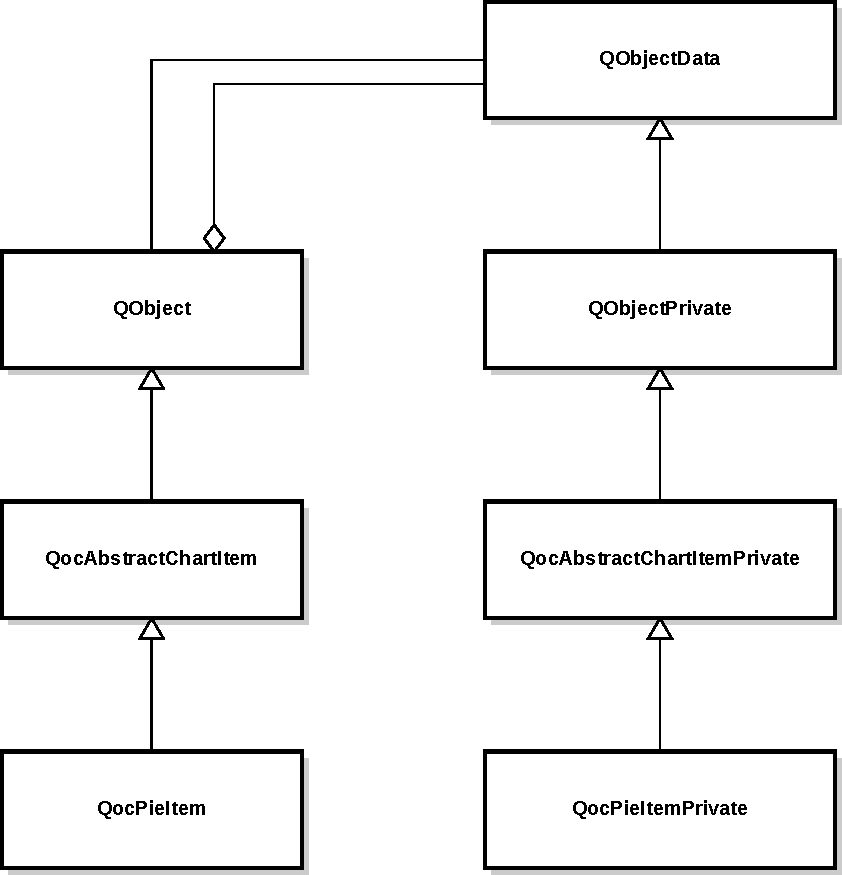
\includegraphics[scale=0.8]{img/dpointer.pdf}
\caption{Przykładowa hierarchia klas}\label{rys:dpointer}
\end{figure}

W~Qt przyjęto następującą koncepcję nazewniczą:
\begin{itemize}
\item{uchwyt ma standardową nazwę, zgodną ze swoim przeznaczeniem,}
\item{ciało ma nazwę składającą się z~nazwy odpowiadającego mu uchwytu oraz sufiksu ,,Private''.}
\end{itemize}


\subsection{Dostęp do uchwytów i ciał}
Podejście opisane w~poprzednim punkcie skutkuje jednak powstaniem pewnego efektu ubocznego.
Wskaźniki do uchwytu i~ciała są typów klas znajdujących się na szczycie hierarchii dziedziczenia. Dostęp do metod klas pochodnych niewystępujących w~klasach bazowych wymaga rzutowania w~dół. 
Problem ten rozwiązano za pomocą czterech makrodefinicji przyjmujących jako argument nazwę klasy uchwytu. Dwie z~nich należy wywołać w~odpowiednich nagłówkach. Z~kolei pozostałe dwie należy wywoływać na początku każdej metody wymagającej odwołania do ciała lub uchwytu. Miejsce wykorzystania konkretnych makr podaję w~tablicy~\ref{tab:makra}. Technika ta została szczegółowo opisana w~artykule~\footnote{QObject -- Most \url{http://qt-project.org/wiki/Dpointer}}

\begin{table}[h]\footnotesize
\centering
\caption{Makrodefinicje}
\label{tab:makra}
\begin{tabular}{|c|c|c|}
\hline
Miejsce & Uchwyt & Ciało\\
\hline
Nagłówek & Q\_DECLARE\_PRIVATE & Q\_DECLARE\_PUBLIC\\
\hline
Metoda & Q\_D & Q\_Q\\
\hline
\end{tabular}
\end{table}
